\newif\ifvimbug
\vimbugfalse

\ifvimbug
\begin{document}
\fi

\exercise{Neural Networks}
In this exercise, you will use the dataset \texttt{mnist\_small}, divided into four files. The \textit{mnist} dataset is widely used as benchmark for classification algorithms. It contains 28x28 images of handwritten digits (pairs \texttt{<input, output>} correspond to \texttt{<pixels, digit>}).

\begin{questions}

%----------------------------------------------

\begin{question}{Multi-layer Perceptron}{20}
Implement a neural network and train it using backpropagation on the provided dataset. Choose your loss and activation functions and your hyperparameters (number of layers, neurons, learning rate, ...), briefly explaining your choices. You \textbf{cannot} use any library beside \texttt{numpy}! That is, you have to implement by yourself the loss and activation functions, the backpropagation algorithm and the gradient descent optimizer (if you want to use any).

Show how the misclassification error (in percentage) on the testing set evolves during the learning. An acceptable solution achieves an error of 8\% or less. Attach snippets of your code. 

Hint: if your network does not learn, check how the network parameters change and plot the trend of your loss function.

\begin{answer}
For the activation function I chose the sigmoid activation function. I choosed this activation function, since its derivation can be formulated using the actual function (logistic differntial equation). This makes implementing gradient descent very easy. However since I choose this approach, it is non-trivial to change the activation function, since its derivative is hardcoded in the gradient descent algorithm.
\begin{equation}
	g(x)=\frac{1}{1+e^{-x}}
\end{equation} 
\begin{equation}
	\frac{d}{dx}g(x)=g(x)\cdot (1-g(x))
\end{equation}

For the loss function I simply try to minimize between the output $f(x,w)$ of the neural network and the label $y$. For this purpose a one-hot-encoding is used. 
\begin{equation}
	L=y-f(x,w)
\end{equation}

For the number of layers I went with a single layer. One layer should be sufficient enough to achieve the given metric. It is also easy to train and easy to implement. 

The number of neurons, learning rate and epoch count are chosen after my feeling of what could potentially work. 

If we now have a look at the graph showing the error on the validation set, we can see that it decreases with each epoch and reaches a minimum at 5.38 percent \ref{fig:nn}. 
\end{answer}
\begin{figure}[H]
	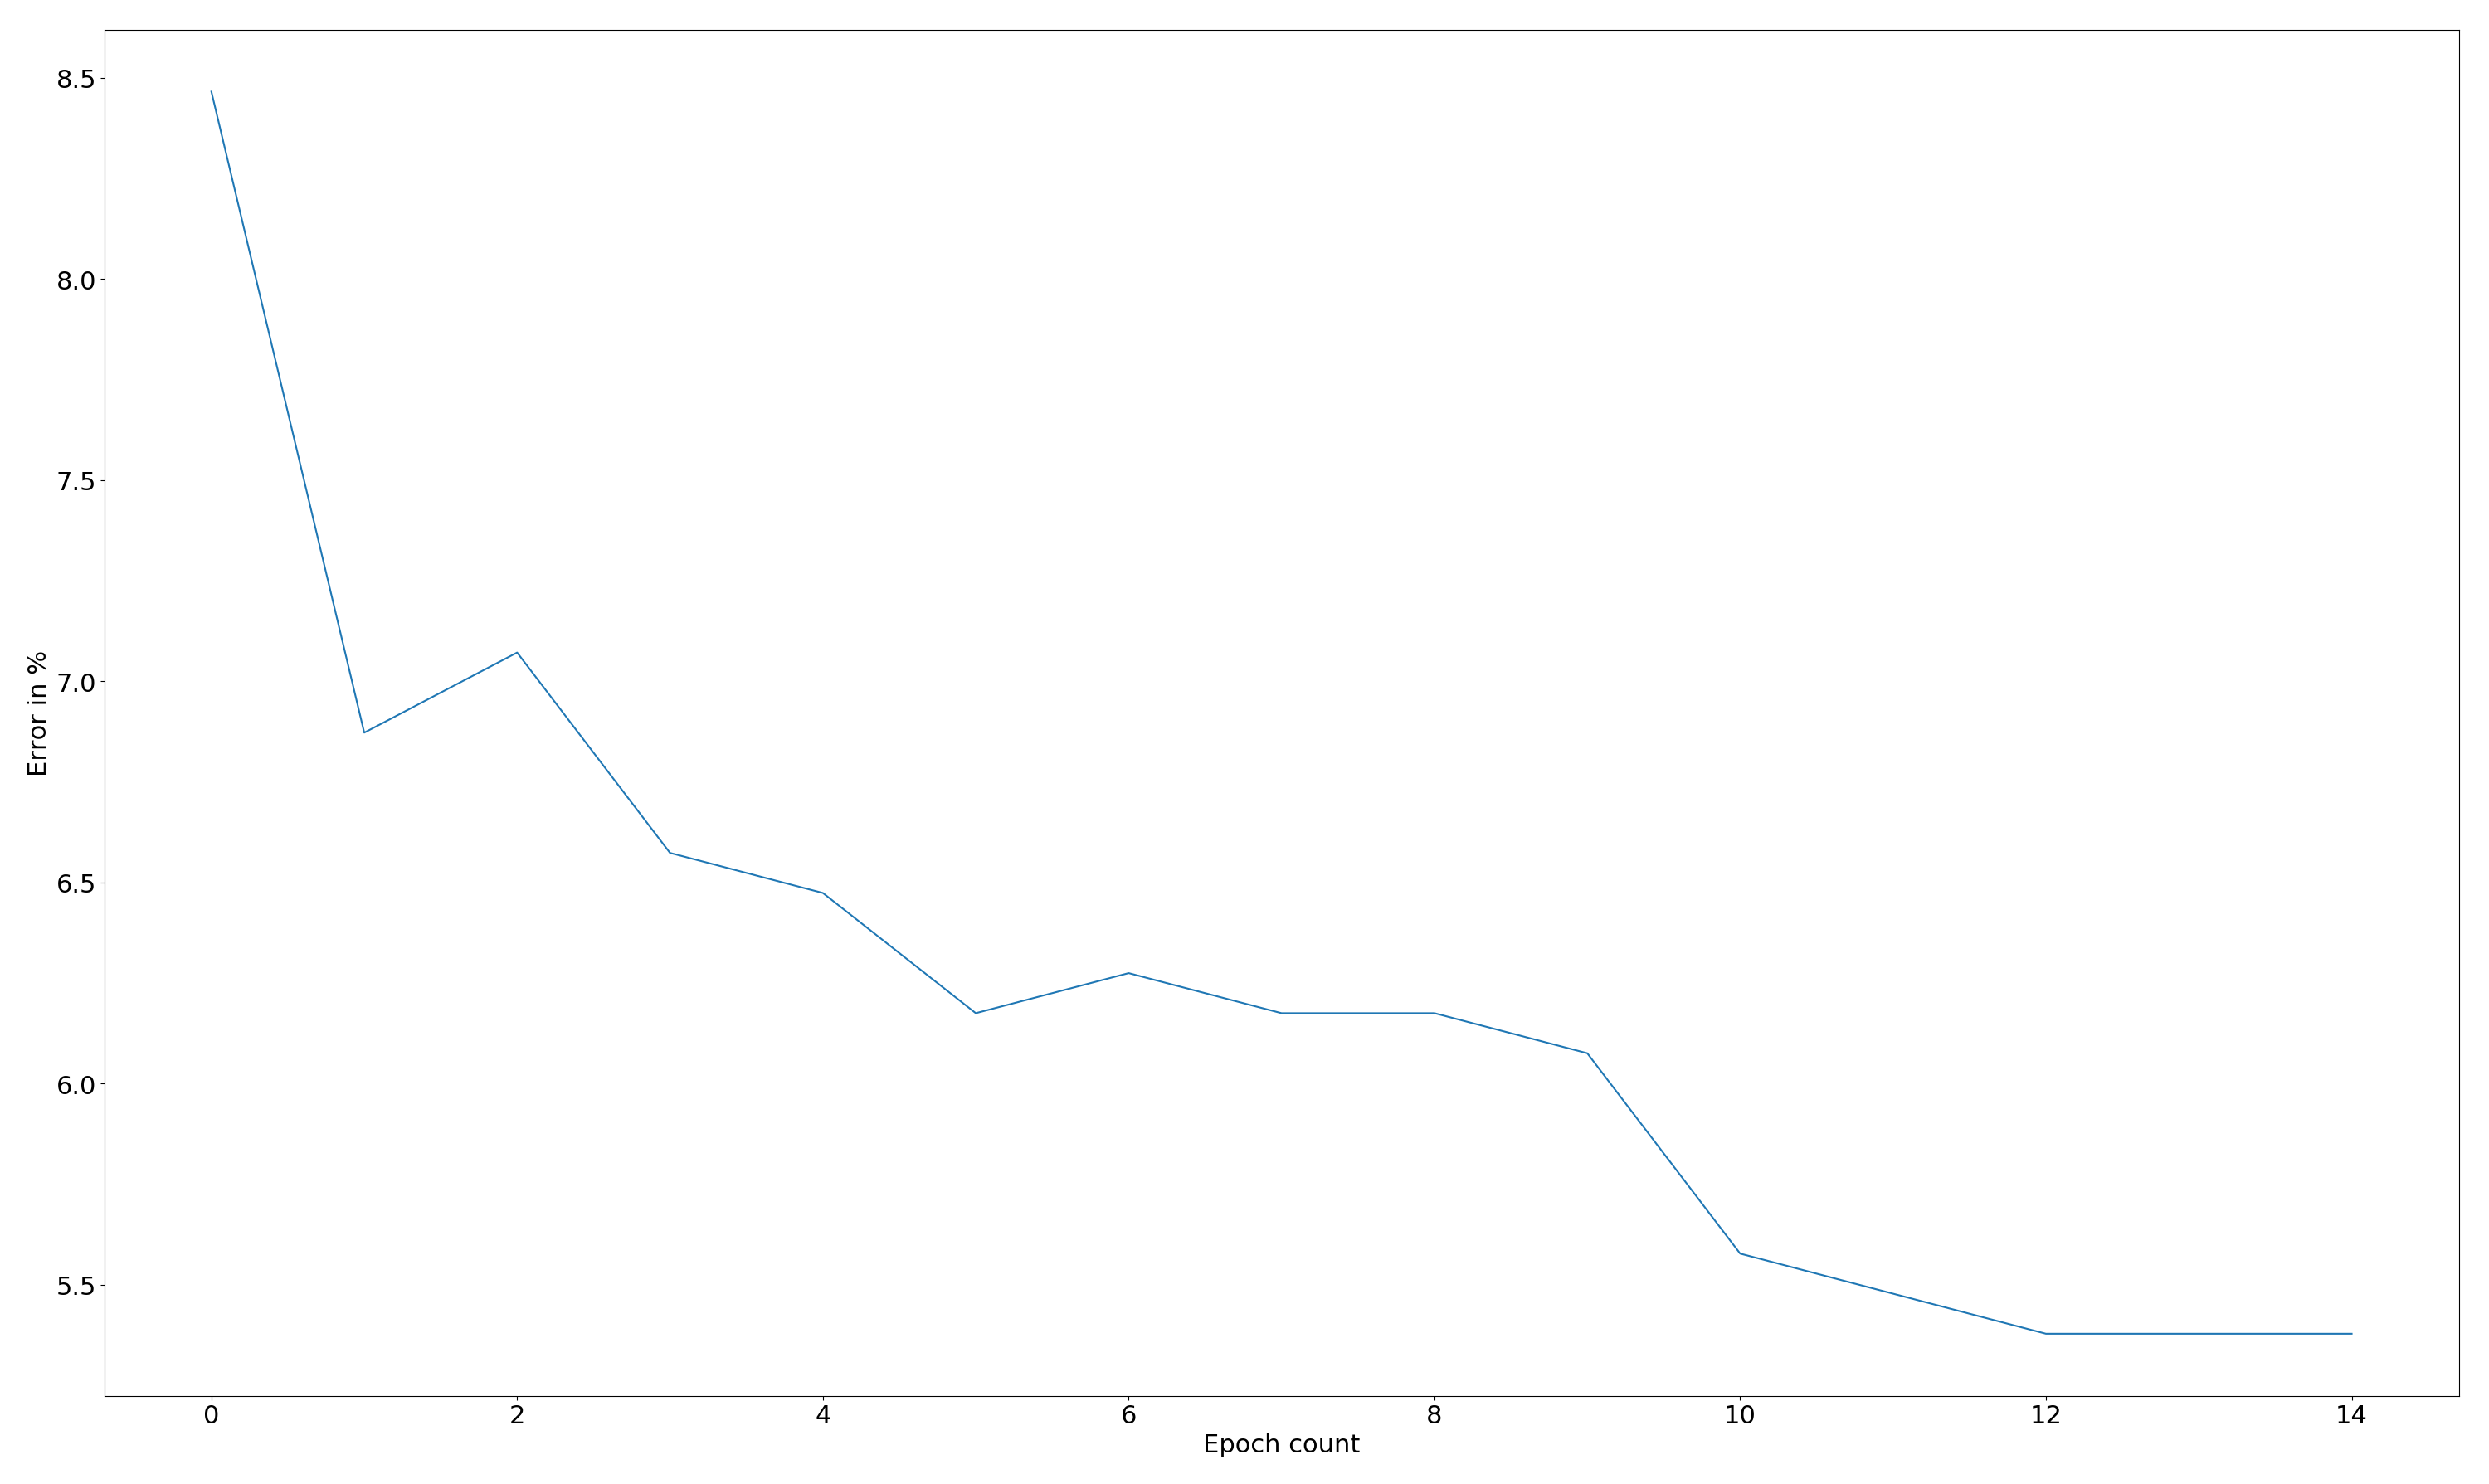
\includegraphics[width=0.8\linewidth]{pictures/NN_loss.png}
	\centering
	\caption{Classification error of the Neural Network for each epoch.}
	\label{fig:nn}
\end{figure}

Since I have already written a Neural Network last year, the code is mostly reused from that time, with removed scipy dependencies. I learned about Neuronal Networks from Tariq Rashid, so parts of my codes will borrow from his implementation. I also had some problems loading the train/test-in data with numpy, so I put them in excel and saved them again as csv, which made them work. Since this mnist dataset is sorted we need to shuffle them. I found a nice numpy function on stackoverflow which does exactly that. 
\lstinputlisting[language=Python]{code/Neural_Network.py}
\end{question}

%----------------------------------------------

\begin{question}[bonus]{Deep Learning}{5}
In recent years, deep neural networks have become one of the most used tools in machine learning. 
Highlight the qualitative differences between classical neural networks and deep networks. Which limitations of classical NN does deep learning overcome?
Give an intuition of the innovations introduced in deep learning compared to traditional NN.
(Hint: Have a look \href{http://arxiv.org/abs/1206.5538}{at this paper}. Use Google Scholar to read other scientific papers for more insights.)

\begin{answer}
The main qualitative difference between classical neural networks and deep networks is the number of layers used. Classical neural networks mostly used only a single layer. This was due to the fact that training deeper structures was hard because of vanishing gradients and considered uncesseray since the universal approximation theorem states that a single hidden layer is enough. This in combination with less training data and avaiable gpu power led to only focus on training single layer neuronal networks. 

One of the main pitfalls of classical neuronal networks was not thinking about the futher consequences of the universal approximation theorem. As it turns out, even if a single layer neural network can learn every function, the theorem doesn't state the complexity needed thus resulting in massive overfitting. 

When talking about learning representations in machine learning one key aspect is the hierachical organization of explanatory features. This means that concepts can can be defined in terms of other concepts which are all placed in a hierarchy. The more abstract, non-linear concepcts are at the top of the hierarchy. This allows Deep neural network to build more abstract features in the high levels on top of other features. In a sense a deep neural network is nothing more than a giant feature building machine. 

Another strong point for the neural network is that it allows for the re-use of features. This property exists thanks to an exponential grow in the number of paths in the circuit that arise in deeper models. 


\end{answer}

\end{question}

%----------------------------------------------

\end{questions}
